\documentclass[pdftex,12pt,a4paper]{report}

\usepackage[pdftex]{graphicx}
\usepackage{enumitem}
\usepackage{fmtcount}
\usepackage{multirow}
\usepackage[margin=0.8in]{geometry}
\usepackage{verbatim}
\usepackage{moreverb}

\renewcommand{\thefootnote}{\arabic{footnote}}
\newcommand{\HRule}{\rule{\linewidth}{0.5mm}}

\begin{document}


\begin{titlepage}
\begin{center}

\begin{minipage}{0.4\textwidth}
\begin{flushleft}

\includegraphics[width=0.6\textwidth]{./logo_telecom.jpg}
\end{flushleft}
\end{minipage}
\begin{minipage}{0.4\textwidth}
\begin{flushright} \large

\includegraphics[width=0.7\textwidth]{./arm.jpg}\\
ARM Ltd. \\                                                                
110 Fulbourn Road \\
Cambridge \\
GB-CB1 9NJ \\
Great Britain \\
\end{flushright}
\end{minipage}\\[1.5cm]

% Upper part of the page

\includegraphics[width=0.3\textwidth]{./mbed.jpg}\\[1.5cm]

\LARGE Industrial Placement Report\\[0.5cm]
% Title
\HRule \\
{ \huge \bfseries Embedded systems: \\ From a local connectivity to the cloud}\\

\HRule \\[1cm]

% Author and supervisor
\begin{minipage}{0.4\textwidth}
\begin{flushleft} \large
\emph{T\'{e}l\'{e}com Paristech mentor:}\\
Samuel \textsc{Tardieu}
\end{flushleft}
\end{minipage}
\begin{minipage}{0.4\textwidth}
\begin{flushright} \large
\emph{Supervisor:} \\
Simon \textsc{Ford}
\end{flushright}
\end{minipage}\\[1.0cm]


\begin{minipage}{0.4\textwidth}
\begin{center} \large
\emph{Author:} \\
Samuel \textsc{Mokrani}
\end{center}
\end{minipage}\\[3.0cm]

\large This report summarises the work I did during my T\'{e}l\'{e}com ParisTech engineering internship. I worked at ARM, more precisely in the Mbed team, from the 4th of July 2011 until the 3rd of February 2012.



\vfill

% Bottom of the page
{\large \today}

\end{center}

\end{titlepage}
\tableofcontents
\chapter{ARM and Mbed}
\section{ARM}
ARM Holdings plc is a British multinational semiconductor and software company. The headquarter is based in Cambridge. This company is well-known in the processor field, although it also designs, licenses and sells software development tools under the RealView and KEIL brands, systems and platforms, system-on-a-chip infrastructure and software. 
\\

Advanced RISC Machines Ltd (now ARM Ltd) was founded in November 1990. It is the result of a joint venture between Acorn Computers, Apple Computer (now Apple Inc.) and VLSI Technology (now NXP semiconductor). The purpose of this joint venture was to develop a RISC chip originally developped by Acorn Computer involved in an Apple project. ARM got bigger little by little by acquiring companies like Micrologic Solutions, a software consulting company based in Cambridge 1999. In 2000, ARM acquired Allant Software, Infinite Designs in Sheffield (UK) and EuroMips in Sophia Antipolis (France). Then, in 2001, it acquired a team specialized in hardware and software debugging based in Blackburn (UK). In 2005, ARM acquired Keil Software, a leader in the software development tools for microcontrollers. More recently, ARM joined with Texas Instrument, Samsung, IBM, ST-Ericsson and Freescale Semiconductor in forming an open source engineering company named Linaro. Linaro produces for example ARM tools or linux kernels for ARM based system-on-chips. Today, ARM has offices and design centres all over the world, including UK, Germany, France, Israel, Sweden, Norway, Slovenia, USA, China, South Korea, Japan, Taiwan and India. 
\\

Nowadays, ARM processors are widely used in mobile phones, tablets, personal digital assistants, GPS, digital cameras and digital televions. The main reason of this success is their low electric power consumption; making them suitable for embedded systems. Even if ARM products are widely used, the company doesn't manufacture its own CPUs. The company licenses its technology as Intellectual Property (IP). Companies like Intel, Texas Intrument or Nvidia are making processors based on ARM's IP.



\section{Mbed}
In wish to pursue new areas of expertise, ARM founded Mbed in 2009. Mbeds core area is development of prototyping boards (called mbed) based on ARM processors (Cortex M0 and Cortex M3). The purpose is to make available a simple and easy to set-up prototyping solution using 32-bits processors. Mbeds boards have been designed for quick experimentation. Users can try something and see if it is doable in a very easily and quickly manner.

\subsection{Mbed boards}
For the moment, three boards have been developped. The first one is based on the LPC2368 microcontroller from NXP which uses a Cortex m3. The second is based on a LPC1768 (Cortex m3). More recently, a new board based on a LPC11U24 (Cortex m0) was born. This last mbed has been particularly designed to prototype USB devices or battery powered applications. 

\begin{figure}[h!]
\centering
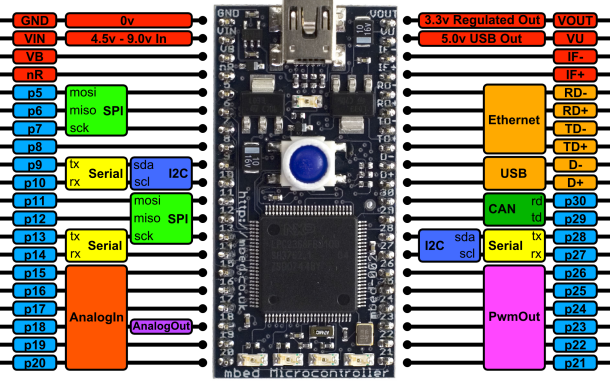
\includegraphics[width=0.5\textwidth]{./lpc1768.png}
\caption{mbed board: lpc1768 (cortex m3)}
\label{mbed_board: lpc1768 (Cortex m3)}
\end{figure}

\begin{figure}[h!]
\centering
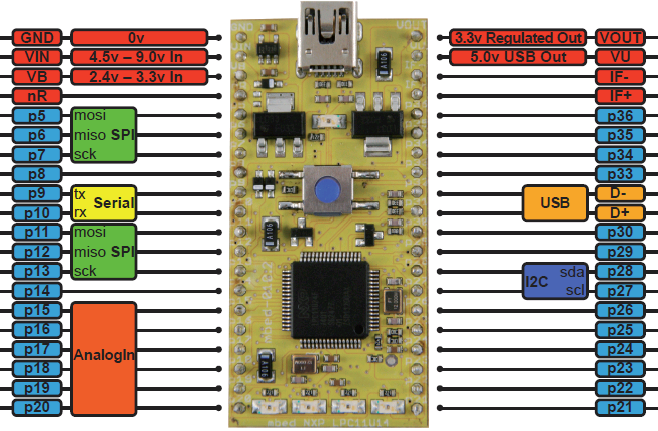
\includegraphics[width=0.5\textwidth]{./lpc11U24.png}
\caption{mbed board: lpc11U24 (cortex m0)}
\label{mbed_board: lpc11U24 (Cortex m0)}
\end{figure}


\subsection{The online compiler}
The two main keywords of Mbed are "simple" and "cloud computing". Users indeed use an online compiler to develop their program in C++. They compile online and transfer the binary received into the mbed, which is connected to a computer over a USB cable and detected as a mass storage device. They just have to press the reset button to see their program running.
\\

As explained before, users have a complete online IDE totally independant of the underlying operating system. 
This IDE has a lot of very interesting features:
\begin{itemize} \itemsep 0em
	\item Code editing with syntax highlighting
	\item Multiple programs
	\item Import programs from online catalogue of published programs
	\item Import programs from zip file
	\item Full output of compile-time messages
	\item Multiple target support
	\item Publish your code directly from the compiler
	\item Export your programs as a .zip file
	\item Build information including graphical display of code size and RAM usage
	\item Code formatter
	\item Import and update of libraries from SVN
	\item Version control: you can commit, revert, update, merge your programs
\end{itemize}

\subsection{Mbed libraries}
In addition to the online compiler, almost all drivers have been implemented. Users just have to instanciate an object such as SPI, I2C,... to have access to a great API which abstract all the low-level layer. \\


\begin{figure}[h!]
\centering
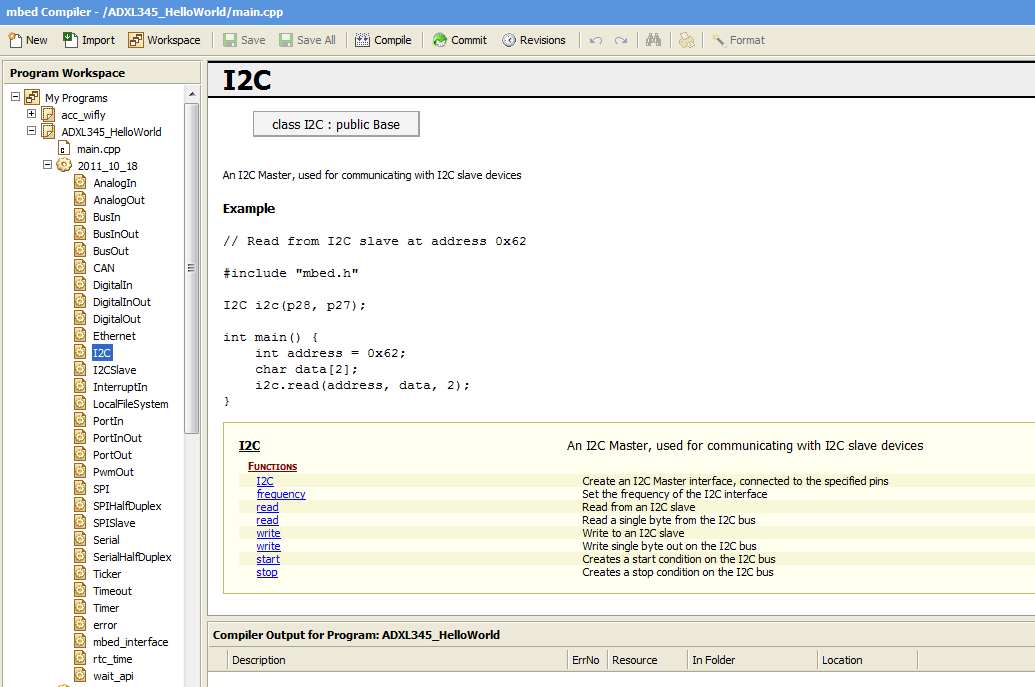
\includegraphics[width=0.7\textwidth]{./libraries.png}
\caption{mbed libraries}
\label{mbed libraries}
\end{figure}


\subsection{Mbed website: \textit{http://mbed.org/}}
To finish this tour of the mbed environment, users can find an active website. First, users have access to a forum. They have also access to a handbook where there is a lot of documentation and examples concerning mbed libraries, the hardware part of the mbed,... But the most important feature of this website is for me the central cookbook. This cookbook is a great source of example coming from other mbed users. You can almost find for instance a lot of libraries to use popular sensors like accelerometers, pressure sensors,... Each user is free to contribute to this part of the website by doing articles explaining their project. 

\begin{figure}[h!]
\centering
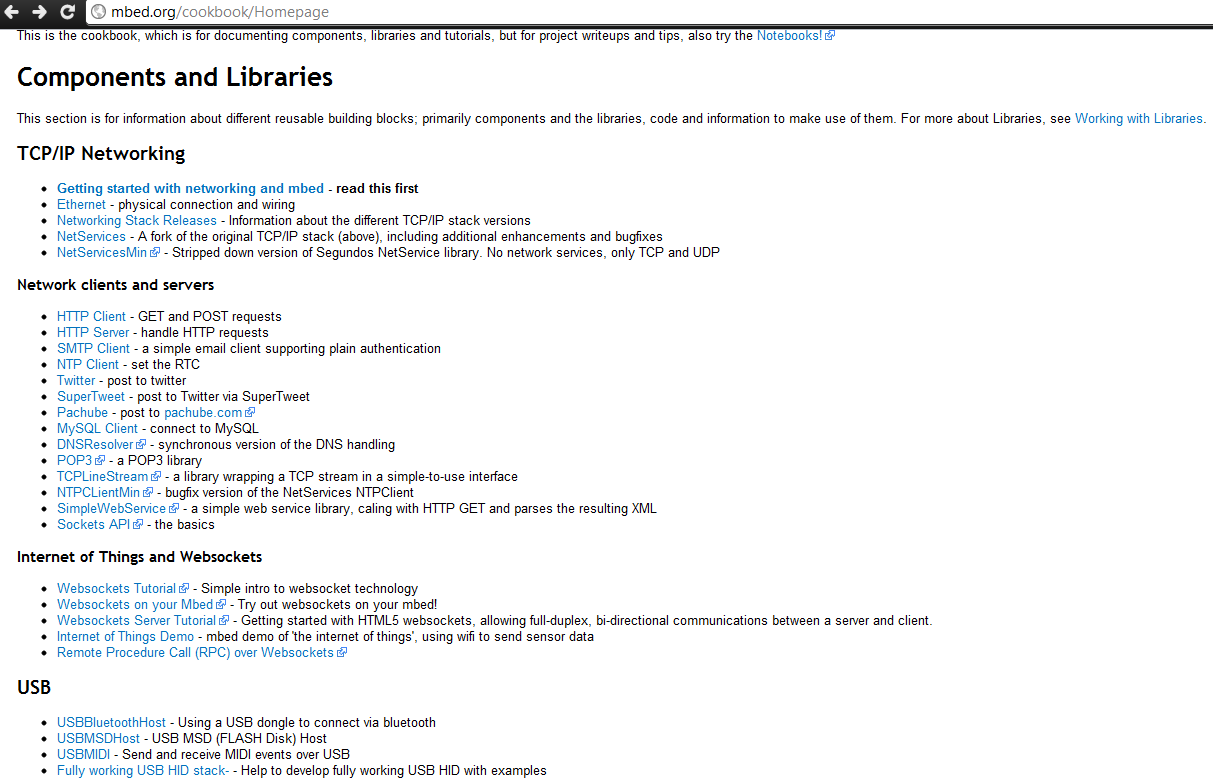
\includegraphics[width=0.7\textwidth]{./cookbook.png}
\caption{mbed cookbook}
\label{mbed cookbook}
\end{figure}


\chapter{Internet Of Things: internet device boom}
Nowadays, an increasing number of devices are connected to the Internet. These devices include not only personal computers, but also mobile phones and digital televisions, ect.
Cisco predicts in an interview from the BBC that the number of internet connected devices is set to explode in the next four years to over 15 billion - twice the world's population by 2015. And Cisco is not the only one company to predict a such boom. VMware's CEO Paul Maritz said during a speech at the annual VMworld conference in Las Vegas in August 2011 that:

\begin{quote} "Three years ago over 95 percent of the devices connected to the Internet were personal computers. Three years from now that number will probably be less than 20 percent. More than 80 percent of the devices connected to the Internet will not be Windows-based personal computers." \\
\end{quote}

Thus, working on the connection of different sensors to the Internet is becoming more and more crucial. I will describe in this chapter two projects concerning the Internet of Things: real-time data streaming from sensors and Remote Procedure Call mechanism. Both of these projects use a new feature of HTML5: a Webscoket communication.

\section{Websockets}
\subsection{Introduction}
The WebSocket specification is a new feature of HTML5. It defines a full-duplex single socket connection over which messages can be sent between client and server. The WebSocket standard simplifies much of the complexity around bi-directional web communication and connection management. Furthermore, it reduces polling and unnecessary network throughput overhead. 

\begin{figure}[h!]
		\centering
		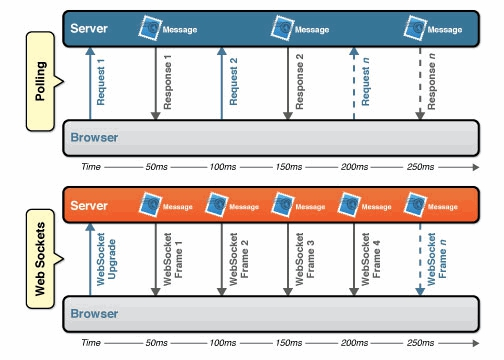
\includegraphics[width=0.7\textwidth]{./ws_poll.jpg}
		\caption{Reduction of polling and overhead by Websocket \textit(Image coutesy of Kaazing)}
		\label{Reduction of polling and overhead by Websocket}
\end{figure}

This figure shows the reduction in latency. Once the connection is established, messages can flow from the server to the browser. As the connection remains open, there is no need to send another request to the server.

\subsection{Websocket protocol}

To establish a WebSocket connection, the client and server upgrade from the HTTP protocol to the WebSocket protocol during their initial handshake. There are several handshake mechanisms. Here I present the basic handshake of one of them; the websocket protocol 76, which has been  implemented in mbed websocket library:


The handshake from the client looks as follows: \\

\fbox{\begin{minipage}{1.0\textwidth} \small
	GET /ws HTTP/1.1 \\
	Host: example.org \\
  Connection: Upgrade \\
  Sec-WebSocket-Key2: 12998 5 Y3 1  .P00 \\
  Upgrade: WebSocket \\
  Sec-WebSocket-Key1: 4 @1  46546xW\%0l 1 5 \\
  Origin: http://example.org \\ \\
  \^{}n:ds[4U
  \end{minipage}
}
\\ \\
The handshake from the server looks as follows: \\

\fbox{\begin{minipage}{1.0\textwidth} \small
        HTTP/1.1 101 WebSocket Protocol Handshake \\
        Upgrade: WebSocket \\
        Connection: Upgrade \\
        Sec-WebSocket-Origin: http://example.org \\
        Sec-WebSocket-Location: ws://example.org/ws \\ \\
        8jKS'y:G*Co,Wxa-
        \end{minipage} 
        }
\\ \\
Once the Websocket connection is established, data can be exchanged according to this format:
\begin{itemize} \itemsep 0em
	\item Send a 0x00 byte
	\item Encode the message using UTF-8 and send the resulting byte stream
	\item Send a 0xFF byte
\end{itemize}

\subsection{Architecture of a Websocket communication}
A websocket communication involves several clients connected to the same websocket server. All messages from browsers are sent to the server. The server manages all messages. It can decide to send a message received from a client to another client, to broadcast all messages received to all clients connected,...


\begin{figure}[h!]
		\centering
		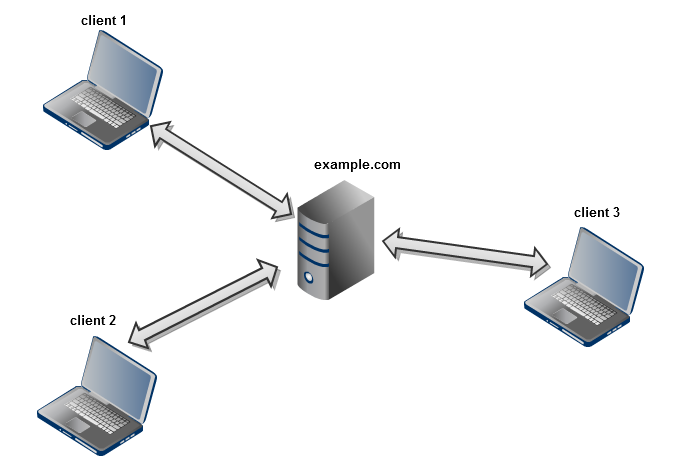
\includegraphics[width=0.7\textwidth]{./ws.png}
		\caption{Example of websocket communication}
		\label{Example of websocket communication}
\end{figure}


For instance, let's say that there is an existing websocket server: example.com which is listening on port 80. A client can open a connection, receive and send messages to this server with this few lines of javascript:

\begin{center}
\begin{boxedverbatim}
var ws = new WebSocket("ws://example.com");
ws.onopen = function(evt) { 
   alert("Connection open"); 
   ws.send("Hello")}; 
};
ws.onmessage = function(evt) { 
   alert( "Message received: " + evt.data); 
}; 
ws.onclose = function(evt) { 
   alert("Connection closed."); 
};
\end{boxedverbatim}
\end{center}



\section{Real-Time Streaming Data from sensors}
\section{Remote procedure Call over Websockets}
	
	
	
	
	
	
	
	
	
	
	
	
	
	
	
	
	
	
	
	
	
	
	

\chapter{Universal Serial Bus}
\section{USB overview}
The Universal Serial Bus (USB) is the most widely used bus in today's computer. USB has particularly been designed to standardize connections between the computer and peripherals. For instance, keyboards, printers, scanners, disk drives or cameras can use the same bus to exchange data with a computer. USB has effectively replaced a variety of earlier interfaces, such as serial or parallel ports. The most useful advantage is certainly the plug-and-play nature it has. In other words, you can connect and disconnect devices on your computer without the need to restart it.\\

USB version 1.1 supported two speeds, a full speed mode of 12Mbits/s and a low speed mode of 1.5Mbits/s. USB 2.0, which is the most widely version of USB, can reach 480Mbits/s. The 480Mbits/s is known as High Speed mode. USB version 3.0 specifies a maximum transmission speed of up to 5Gbits/s (known as SuperSpeed), however few products are supporting USB 3.0 at present.
\\
\begin{table}[h!]
\begin{center}
\begin{tabular}{|l|l|l|}
\hline
\multirow{2}{*}{USB 1.1} & low-speed & 1.5Mbits/s \\
 & full-speed & 12Mbits/s \\ \hline
USB 2.0 & high-speed & 480Mbits/s \\ \hline
USB 3.0 & super-speed & 5Gbits/s \\ \hline
\end{tabular}
\end{center}
\caption{USB speeds}
\label{USB speeds}
\end{table}

The Universal Serial Bus is host controlled. However, there can only be one host per bus and the host is responsible for undertaking all transactions. Considering this restriction, two devices cannot exchange information without one host. Nevertheless, the On-The-Go specification, which is part of the USB 2.0 standard, has introduced a Host Negotiation Protocol, allowing two devices to negotiate for the role of host. With this specification, we can imagine a camera exchanging data with a printer without the need of a computer. 

\section{How does the USB work?}
\subsection{Topology}
The physical bus topology defines how USB devices are connected to the host. The USB network is implemented as a tiered star network with one host (master) and several devices (slaves). The topology looks like a tree. In order to increase the number of devices connected, a hub need to be connected to the root port. This special hub and the root port are the first tier of the network.Furthermore, the USB network can support up to 127 external nodes but the number of tiers does not exceed 7. The following diagram represents a possible connection architecture on a USB bus.


\begin{figure}[h!]
		\centering
		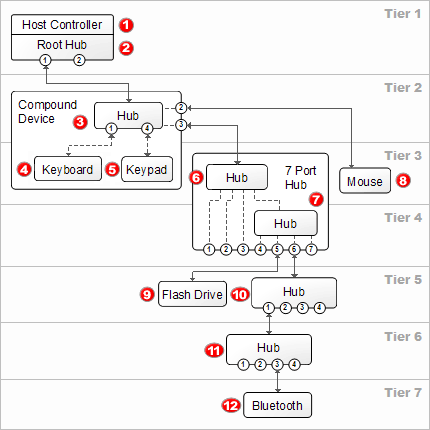
\includegraphics[width=0.5\textwidth]{./usb_topology.png}
		\caption{USB physical topology \footnotemark}
		\label{USB physical topology}
\end{figure}
\footnotetext{reference: http://www.usblyzer.com}
\subsection{Endpoints}
Most devices will have a series of buffers to communicate between the host and the device. Each buffer will belong to an endpoint. An endpoint is a uniquely identifiable entity on a USB device, which is the source or terminus of the data that flows from or to the device. For instance, the mbed based on a NXP LPC1768 microcontroller has 32 physical endpoints whereas the mbed based on the NXP LPC11U24, has 10 physical endpoints. In fact, one physical endpoint represents two logical endpoints. Each physical endpoints has a specific direction: either OUT to receive data from the host or IN to send data to the host. There are four types of endpoints: control, interrupt, bulk and isochronous.
	
\begin{figure}[h!]
		\centering
		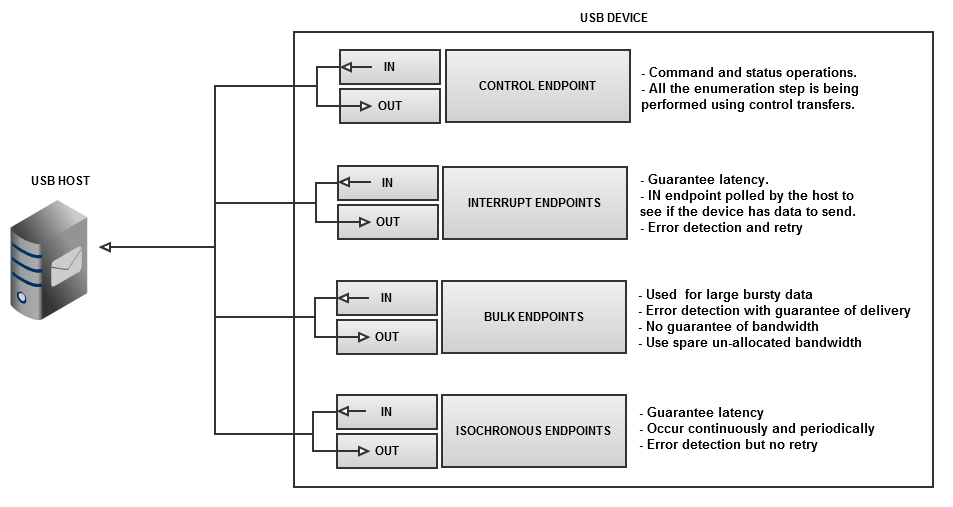
\includegraphics[width=1.0\textwidth]{./endpoint.png}
		\caption{Different types of endpoints}
		\label{Different types of endpoints}
\end{figure}

\newpage

\subsection{Packets exchanged}
\subsubsection{\underline{Common fields in a packet}}

\begin{table}[h!]
\begin{tabular}{|c|c|p{9cm}|}
\hline
Field & Length & Meaningful \\ \hline
\multirow{2}{*}{SYNC} & low and full speed: 8bits  & \multirow{2}{10cm}{A packet starts with a SYNC pattern to allow the receiver bit clock to synchronise with the data.} \\
\cline{2-2}%
 & high speed: 32bits & \\ \hline
 
EOP & 3bits & A packet ends with an End of Packet (EOP) field \\ \hline

PID & 8bits & Packet ID \\ \hline

\multirow{2}{*}{ADDR} & \multirow{2}{*}{7bits} & The address field specifies which device the packet is designated for\\ \hline

\multirow{2}{*}{ENDP} & \multirow{2}{*}{8bits} & The endpoint number which the packet is designed for \\ \hline

\multirow{2}{*}{CRC} & \multirow{2}{*}{5 or 16bits} & Cyclic Redundancy Checks are performed on the data within the packet payload \\ \hline
\end{tabular}
\caption{Fields in a USB packet}
\label{Fields in a USB packet}
\end{table}

\subsubsection{\underline{Packets}}
\begin{itemize}
	\item Token Packet:
		\begin{center}
		\begin{tabular}{|c|c|c|c|c|c|}
  	\hline
  		SYNC & PID & ADDR & ENDP & CRC5 & EOP \\ \hline
  		8/32bits & 8bits & 7bits & 4bits & 5bits & 3bits \\
  	\hline
  	\end{tabular}
  	\end{center}
  	
  	There are three types of token packets: 
  	\begin{itemize} \itemsep 0em
			\item IN: The host wants to read information.
			\item OUT: The host wants to send information.
			\item SETUP: Used to begin control transfers.
  	\end{itemize}
  	
  	
	\item Data Packet:
		\begin{center}
		\begin{tabular}{|c|c|c|c|c|}
  	\hline
  		SYNC & PID & DATA & CRC16 & EOP \\ \hline
  		8/32bits & 8bits & (0 - 1024) * 8bits & 16bits & 3bits  \\
  	\hline
  	\end{tabular}
  	\end{center}
  	
  	
	\item Handshake Packet:
		\begin{center}
		\begin{tabular}{|c|c|c|}
  	\hline
  		SYNC & PID & EOP \\ \hline
  		8/32bits & 8bits & 3bits \\
  	\hline
  	\end{tabular}
  	\end{center}
  	
  	There are four types of token packets: 
  	\begin{itemize} \itemsep 0em
			\item ACK: Packet successfully received.
			\item NAK: The device temporary cannot send or received data
			\item STALL: Endpoint is halted, or control pipe request is not supported.
			\item NYET: No response yet from receiver (high speed only)
  	\end{itemize}
  	
  	
\end{itemize}

\subsection{USB data flow}

\begin{figure}[h!]
		\centering
		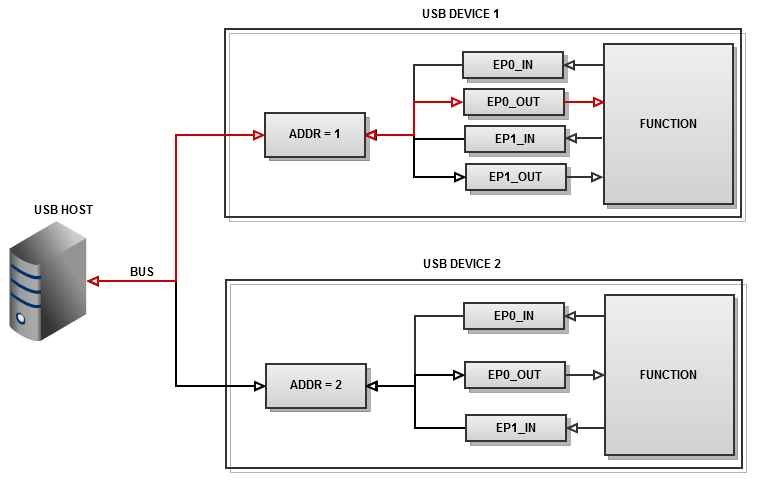
\includegraphics[width=1.0\textwidth]{./data_flow.png}
		\caption{From the host to a device}
		\label{From the host to a device}
\end{figure}

Say for example, the host sends a packet to device=2, endpoint=1OUT. The function hardware will read the request and determine from the address field whether the packet is for itself, and if so will copy the payload of the following data packet to the appropriate endpoint buffer. It will then send a handshake packet to acknowledge the reception of the byte and generate an internal interrupt within the microcontroller for the appropriate endpoint signifying it has received a packet. This is typically all done in hardware.
\\

\subsection{Enumeration}
Once the device plugged into a USB port, the host performs a bus enumeration on the endpoint 0. So, all devices must at least have a control endpoint (endpoint 0) to perform the enumeration step. During this step, the host will assign a unique address to the device. Moreover, descriptors are used to describe a device. A descriptor is just an array containing some information like the device class, the number of endpoints used, the maximum length of these endpoints,... There are several types of descriptors. Standards descriptors are: device descriptor, configuration descriptor, interface descriptor and endpoint descriptor. Besides, for each class, it is possible to have others descriptors like a report descriptor for HID devices.
\\

\begin{figure}[h!]
		\centering
		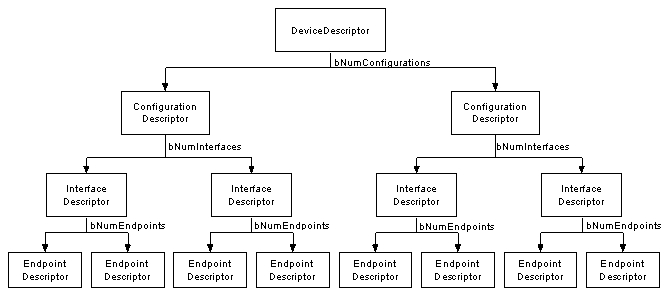
\includegraphics[width=0.7\textwidth]{./descr.jpg}
		\caption{Descriptors}
		\label{Descriptors}
\end{figure}

Enumeration:
\begin{itemize}
	\item GET DEVICE DESCRIPTOR: The host sends a get device descriptor request. The device
replies with its device descriptor to report its attributes (Device Class, maximum packet size for
endpoint zero).
	\item SET ADDRESS: A USB device uses the default address after reset until the host assigns a
unique address using the set address request. The firmware writes the device address assigned by
the host.
	\item GET CONFIGURATION DESCRIPTOR: The host sends a get configuration request. The device replies with its
configuration descriptor, interface descriptor and endpoint descriptor. The configuration
descriptor describes the number of interfaces provided by the configuration, the power source
(Bus or Self powered) and the maximum power consumption of the USB device from the bus.
The Interface descriptor describes the number of endpoints used by this interface. The Endpoint
descriptor describes the transfer type supported and the bandwidth requirements.
	\item SET CONFIGURATION: The host assigns a configuration value to the device based on the
configuration information. The device is now configured and ready to be
used.
\end{itemize}


\newpage
\section{USB Device stack}
A USB device stack has been developped to allow mbed users to design their own USB device or to use their mbed as USB peripheral such as a keyboard or a mouse. USB defines class code information that is used to identify a device�s functionality. This code will be parsed by the USB host stack to load an appropriate device driver. Two widely used USB classes has been implemented: HID (Human Interface Device) and MSD (Mass Storage Device). Users have access to a subset of a third class known as CDC (Communication Device Class). This class is particularly used to design a virtual serial port over USB. The following diagram shows the software architecture of this stack.

\begin{figure}[h!]
		\centering
		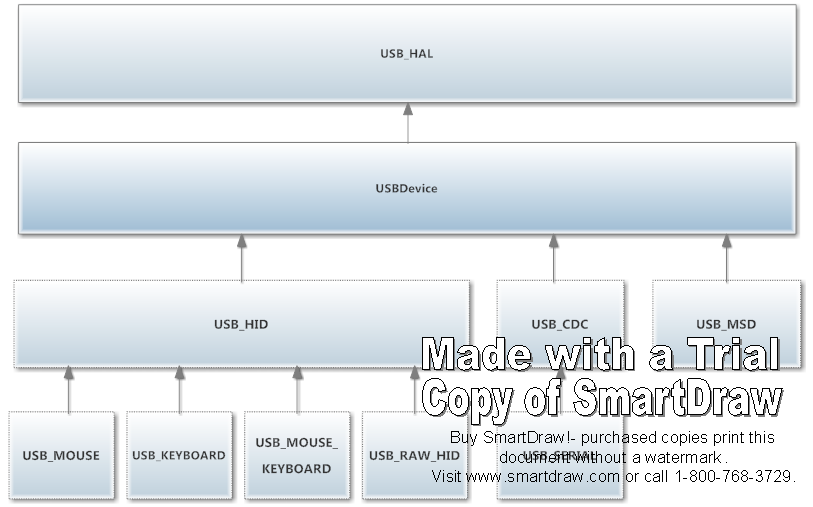
\includegraphics[width=1.0\textwidth]{./usb_stack.png}
		\caption{USB device stack architecture}
		\label{USB device stack architecture}
\end{figure}

As in all stacks, it is organized by layers:
\begin{itemize}
	\item USB\_HAL: The USB hardware layer. All low levels methods are on this class. We found in particular the USB interrupt handler and methods to initialize the USB controller, read or write a certain endpoint. This class defines also virtual methods which are executed each time that there is an interrupt concerning a packet received or the end of a writing. Child classes can use these virtual functions to perform their own treatment when a such event occurs. 	
	\item USB\_DEVICE: This layer is in charge to abstract the hardware. Methods such as USBDevice\_init, USBDevice\_connect, USBDevice\_disconnect, USBdevice\_addEndpoint, USBDevice\_readEndpoint, USBDevice\_writeEndpoint can be found in this class. It's also in this class that the enumeration step is performed for requests concerning standard descriptors. When a packet is received on the control endpoint (endpoint 0), it is decoded to analyze the request and a response to the host is sent. Descriptors are accessible via virtual functions such as getDeviceDescriptor which returns a pointer on the descriptor. As these functions are virtual, all child classes will be able to use their own descriptors.
		\item USB\_HID, USB\_CDC and USB\_MSD: As explained before, these classes represent a specific USB class. A part of the enumeration step can be done here if the host requests a class specific descriptor. These three classes are explained in the next section of this document.
		\item USB\_MOUSE, USB\_KEYBOARD, USB\_MOUSE\_KEYBOARD, USB\_RAW\_HID and \\ USB\_SERIAL: High level libraries to emulate a specific peripheral according to their class. For instance, a keyboard is emulated over the HID class. Methods such as printf, putc are accessible for a keyboard. The USB\_RAW\_HID class is used to send and receive raw data. This can be a good opportunity to design a USB device. USB\_SERIAL is a virtual serial port.
\end{itemize}

\section{HID class}
\section{CDC class}
\section{MSD class}

\section{References}
http://www.bbc.co.uk/news/technology-13613536

\end{document}